
\begin{frame}{Integración continua y desarrollo colaborativo}
\begin{figure}
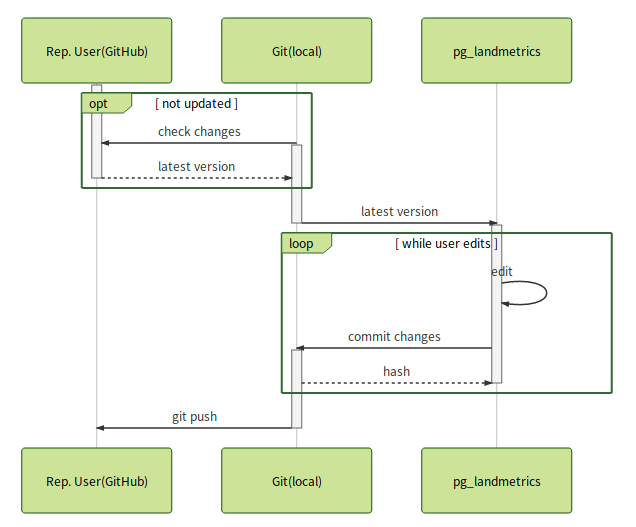
\includegraphics[height=6.5cm]{Metodologia/Figs/diary}
\vspace{-0.5cm}
\caption{\textit{Diagrama de secuencia del flujo de integración continua.}}
\end{figure}
\end{frame}


\begin{frame}{Integración continua y desarrollo colaborativo}
\begin{figure}
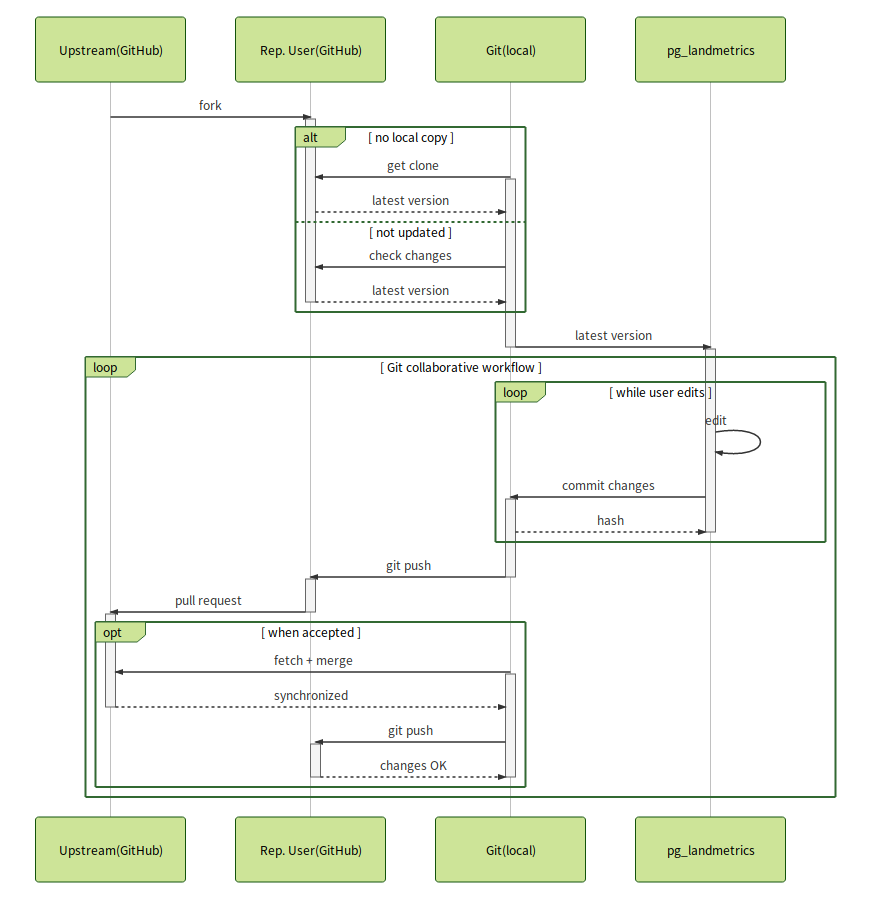
\includegraphics[height=6.5cm]{Metodologia/Figs/pullrequest}
\vspace{-0.5cm}
\caption{\textit{Diagrama de secuencia sobre el desarrollo colaborativo entre repositorios.}}
\end{figure}
\end{frame}


\begin{frame}{Integración continua y desarrollo colaborativo}
\begin{figure}
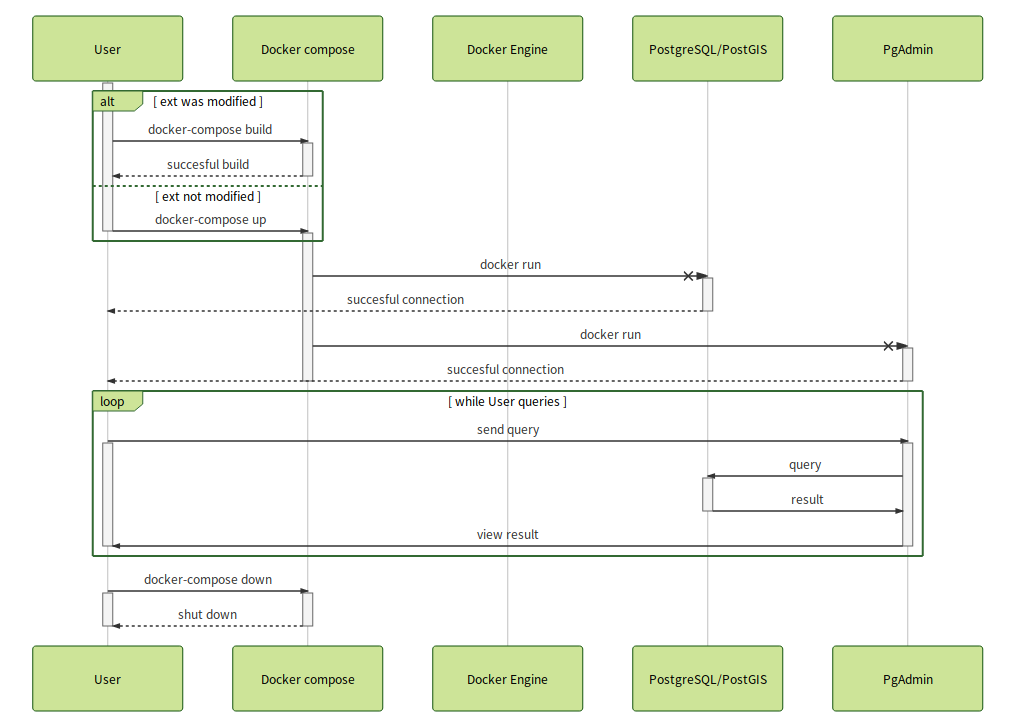
\includegraphics[height=6.5cm]{Metodologia/Figs/ci}
\vspace{-0.5cm}
\caption{\textit{Diagrama de secuencia de implementación y desarrollo de funciones SQL con dockers.}}
\end{figure}
\end{frame}


\begin{frame}{Conjunto de datos}
\begin{figure}
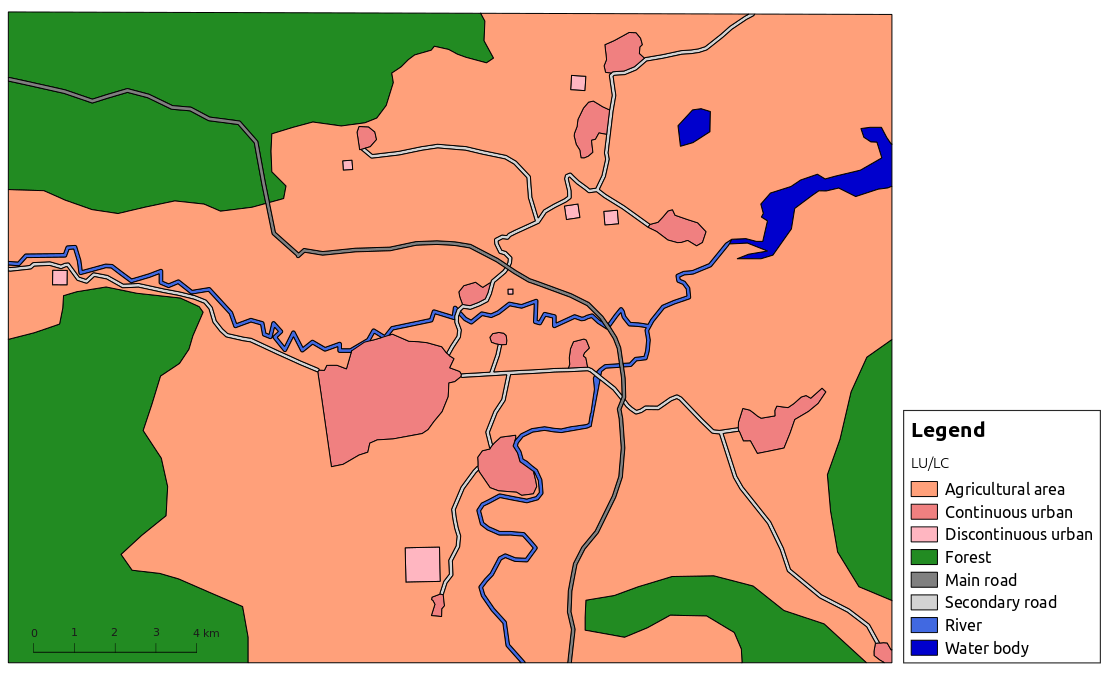
\includegraphics[height=6cm]{Metodologia/Figs/zona_andrea}
\vspace{-0.5cm}
\caption{\textit{Coberturas del suelo del paisaje de ejemplo.}}
\end{figure}
\end{frame}



\frame{
	\frametitle{Conjunto de datos}
	\textit{Características de los conjuntos de datos utilizados:}
	\begin{table}
	\footnotesize
		\renewcommand{\figurename}{Table}
		%\centering
		%\caption{\textit{Características de los conjuntos de datos utilizados.}}
		\begin{tabular}{l l l l}
		\hline
			\textbf{Tipo} & \textbf{Tablas} & \textbf{Filas} & \textbf{Tamaño total} \\ 
			\hline
\multirow{4}{*}{SIOSE-2011}			& t\_nomes        & 36.790.972     & 6116 MB               \\
									& t\_poli\_atrib  & 2.562.800      & 451 MB                \\
									& t\_poli\_geo    & 2.562.800      & 3981 MB               \\
									& t\_valores      & 10.932.639     & 1041 MB               \\ 
            \hline
\multirow{4}{*}{Grids}             & grid\_25k       & 756            & 232,3 kB              \\
								    & grid\_50k       & 192            & 57,8 kB               \\
								    & grid\_100k      & 48             & 13,8 kB               \\
								    & grid\_500k      & 2              & 677bytes              \\ 
			\hline
\multirow{2}{*}{Sample}			    & sample\_25830   & 51             & 122,6 kB              \\
								    & sample\_4326    & 51             & 122,5 kB              \\ 
			\hline
		\end{tabular}
	\end{table}
}




\frame{
	\frametitle{Conjunto de datos}
	%\textit{Métricas de paisaje disponibles en la extensión:}
	\begin{table}
	\tiny
		\renewcommand{\figurename}{Table}
		%\centering
		%\caption{\textit{Características de los conjuntos de datos utilizados.}}
		\begin{tabular}{l l l l}
		\hline
			\textbf{Nivel} & \textbf{Métrica} & \textbf{Abreviatura} \\ 
			\hline
\multirow{8}{*}{Patch}			& Patch Area        						& AREA 			\\
								& Patch Perimeter  							& PERIM 		\\
								& Perimeter-Area-Ratio    					& PARA 			\\
								& Shape Index      							& SHAPE 		\\ 
								& Corea Area       							& CORE 			\\
								& Number of Core Areas  					& NCORE 		\\
								& Core Area Index   						& CAI 			\\
								& Euclidean Nearest Neighbour Distance		& ENN 			\\ 
            \hline
\multirow{8}{*}{Class}         & Total (Class) Area        				& CA 			\\
								& Percentage of Landscape  					& PLAND 		\\
								& Total Edge    							& TE 			\\
								& Edge Density      						& ED 			\\ 
								& Total Corea Area       					& TCA 			\\
								& Core Area Percentage of Landscape  		& CPLAND 		\\
								& Number of Patches   						& NP 			\\
								& Patch Density								& PD 			\\
			\hline
\multirow{9}{*}{Landscape}		& Total Area        						& TA 			\\
								& Total Edge  								& TE 			\\
								& Edge Density    							& ED 			\\
								& Number of Patches      					& NP 			\\ 
								& Patch Density       						& PD 			\\
								& Patch Richness  							& PR 			\\
								& Patch Richness Density   					& PRD 			\\
								& Shannon's Diversity Index					& SHDI 			\\
								& Simpson's Diversity Index					& SHIDI 		\\ 
			\hline
		\end{tabular}
	\end{table}
}





\begin{frame}[fragile]
\frametitle{Desarrollo de funciones en PostgreSQL}
\begin{verbatim}
SELECT siose FROM hoa
\end{verbatim}
\end{frame}



\begin{frame}{Desarrollo de funciones en PostgreSQL}
\begin{figure}
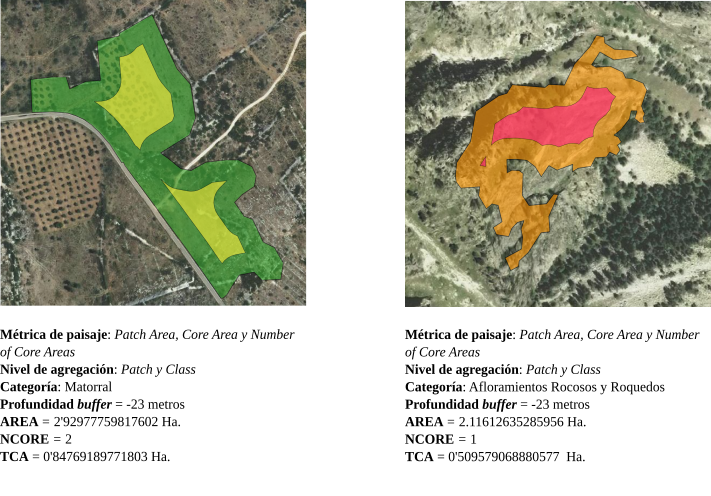
\includegraphics[height=6.5cm]{Metodologia/Figs/figuraejemplo}
\vspace{-0.5cm}
\caption{\textit{Ejemplo de cálculo de AREA, NCORE y TCA a partir de la geometría del SIOSE 2011.}}
\end{figure}
\end{frame}


\begin{frame}{}
Experimento
\end{frame}
